\chapter{Computer Applications}

SuperCollider Programming Language.

\section{Spectral Tracking}
\subsection{PartialTracker}

\begin{verbatim}
	SynthDef.writeOnce(\numpar, {arg fftbuf, magbuf, freqbuf, bus = 1, num = 1, vol = 1;
	var in, chain;
	in = AudioIn.ar(bus, vol);
	chain = FFT(fftbuf, in);
	chain = PV_MaxMagN(chain, num);
	chain = PV_MagBuffer(chain, magbuf);
	chain = PV_FreqBuffer(chain, freqbuf);
	IFFT(chain);
	});
\end{verbatim}

\subsection{FFTFilter}
\subsection{SpearToSC and SpearToMIDI}

\href{http://github.com/freuben/FedeLib/blob/master/SpearToSC/SpearToSC.sc}{SpearToSC} is a SuperCollider class that takes data from the open source software application called  \href{http://www.klingbeil.com/spear/}{SPEAR}\footnote{Michael Klingbeil, SPEAR, 2005, URL: http://www.klingbeil.com/spear/.} and transfers it to an array in SuperCollider. SPEAR uses a variation of the traditional McAulay-Quartieri procedure and ``attempts to represent a sound with many individual sinusoidal tracks (partials), each corresponding to a single sinusoidal wave with time varying frequency and amplitude.''\footnote{Michael Klingbeil, M. 2005. ``Software for spectral analysis, editing, and synthesis.'' in \emph{Proceedings of ICMC}, vol. 2005, 2005. URL: \href{http://www.klingbeil.com/papers/spearfinal05.pdf}{http://www.klingbeil.com/papers/spearfinal05.pdf}.} SPEAR provides a graphical representation of a sound\footnote{Spectral analysis where the y-axis represents frequency in hertz and the x-axis represents time in seconds.} (as seen in Figure 1.1) in which it is possible to select the individual sinusoidal tracks and allows to isolate and access the information for each individual partial. 
\begin{figure}[htbp] %  figure placement: here, top, bottom, or page
   \centering
   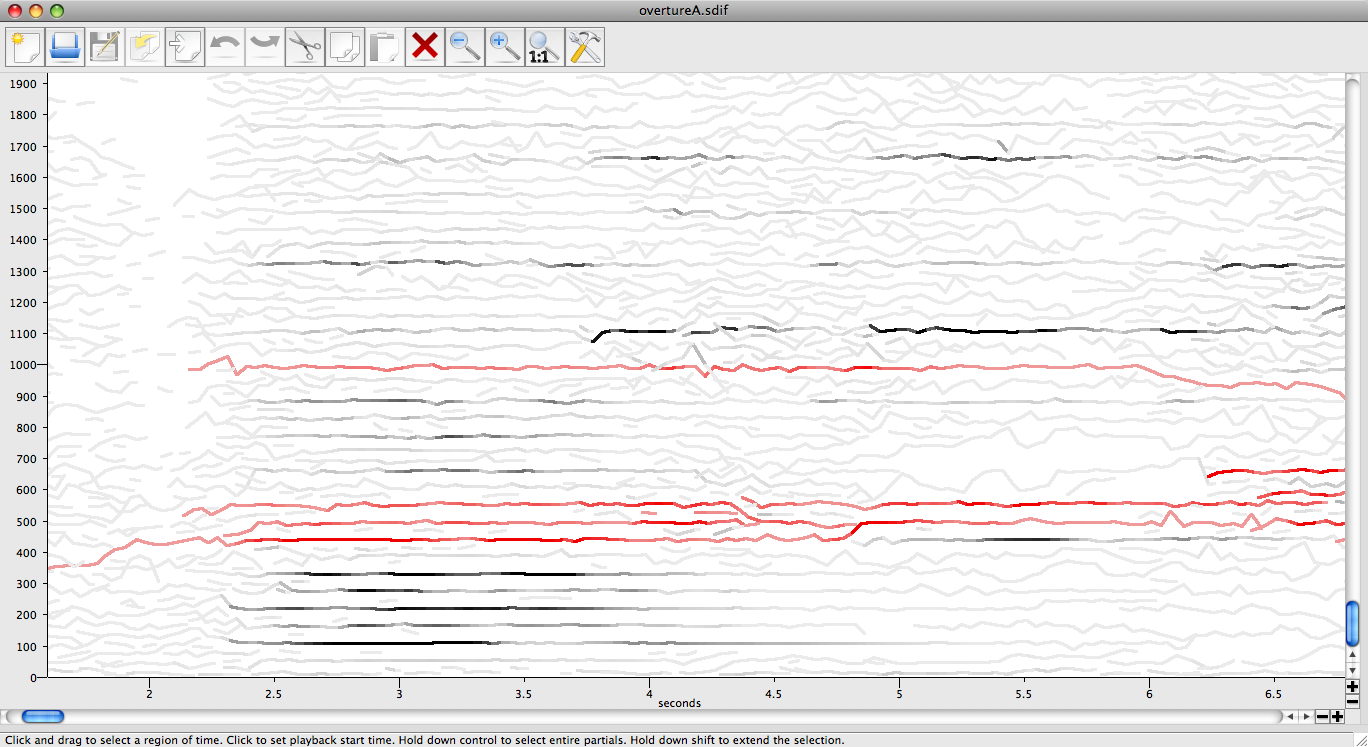
\includegraphics[width=15cm]{Chapter4/Spear1.tif} %change centimeters for resizeing
   \caption{SPEAR graphical interface.}
   \label{fig:example}
\end{figure}
The amplitude and frequency information of each partial given by frame can be stored in a text file. SpearToSC reads text files produced by SPEAR\footnote{SpearToSC reads SPEAR text files in the \emph{Text - Partials} format only.} as a string and strips it into a multidimensional array in SuperCollider. It is therefore possible to process this data within the SuperCollider language and server and re-synthesize this information not only with sinusoidal waves, but with any type of Unit Generator. 

\href{http://github.com/freuben/FedeLib/blob/master/SpearToSC/SpearToMIDI.sc}{SpearToMIDI} reduces the information given by SPEAR to be used as data to produce a MIDI file or to control SuperCollider synthesis definitions. The purpose of this class is to reduce the spectral information to an amount of data that can later produce notated material for a written score, a MIDI file or a control system to be used for triggering synthesis algorithms. The data in the text file generated by SPEAR is available by frame and gives too much information for this purpose. Therefore, the SpearToMIDI class reduces this data in four stages: First, the class takes an amplitude threshold argument which gets rid of all of the partial data that lies bellow this value (as seen in Figure 1.2).
\begin{figure}[htbp] %  figure placement: here, top, bottom, or page
   \centering
   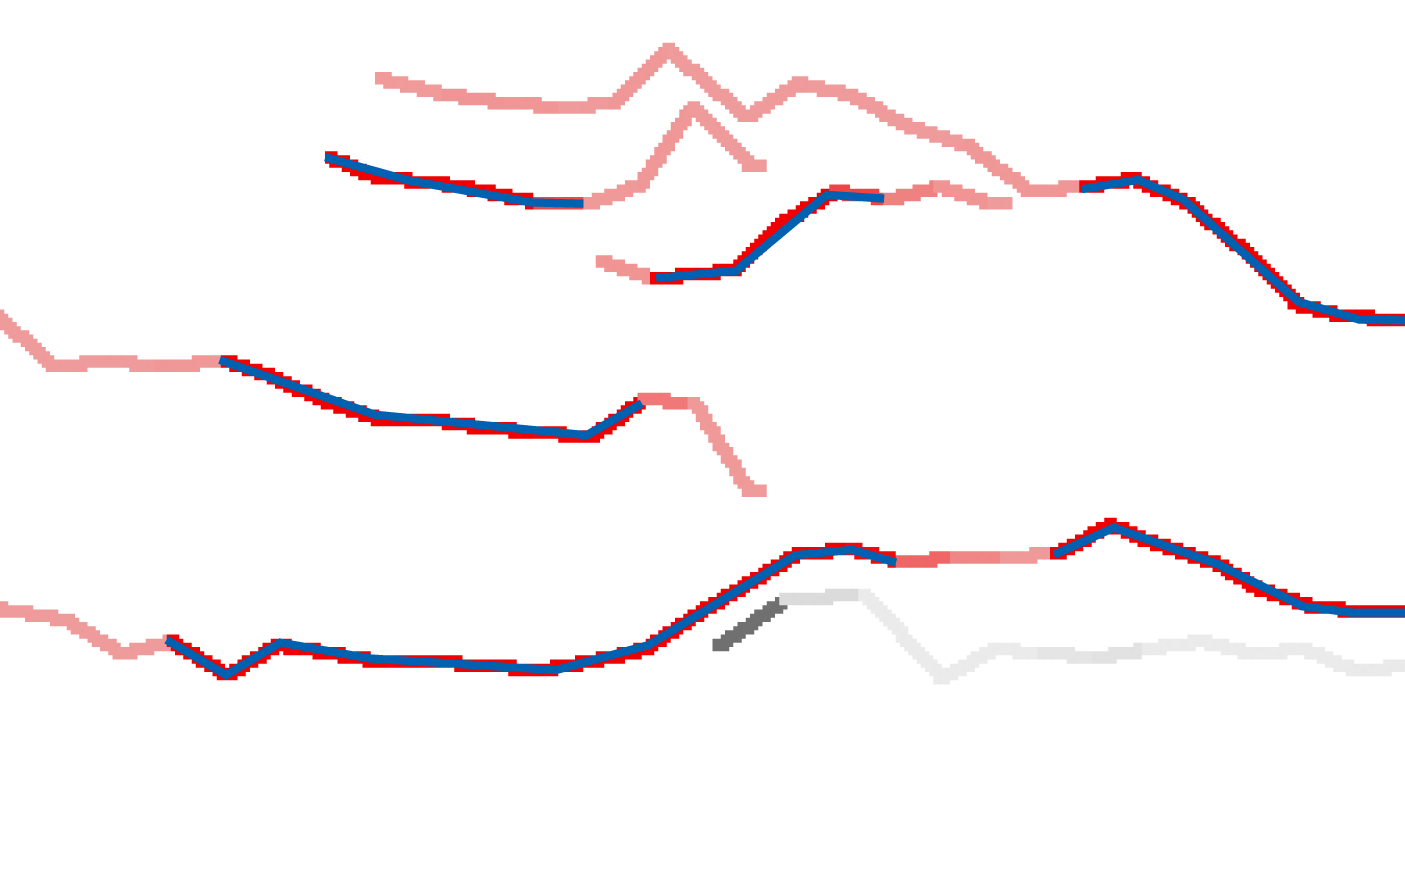
\includegraphics[width=9cm]{Chapter4/Spear2.tif} %change centimeters for resizeing
   \caption{Amplitude threshold selection.}
   \label{fig:example}
\end{figure}\
In other words, it breaks the partial in different groups by introducing silences instead of the data that lies bellow the threshold and at the same time keeps track of the beginning and the end of each group. The second stage reduces data with a frequency modulation threshold. Each group is taken as a line and the computer only stores the points in the line which cross a given interval (the modulation threshold). For example, Figure 1.3 shows how the lines representing the groups in Figure 1.2 are traced by selecting the points that cross a given interval.\footnote{The grid represents the intervals as shown in the y-axis. For the purpose of simplification, the diagram doesn't show a logarithmic representation of frequency.} If the interval is of one semitone then the frequencies are averaged to the closest chromatic note. It is possible to make microtonal divisions of the equal-tempered scale by using floating point values for the note modulation threshold.
\begin{figure}[htbp] %  figure placement: here, top, bottom, or page
   \centering
   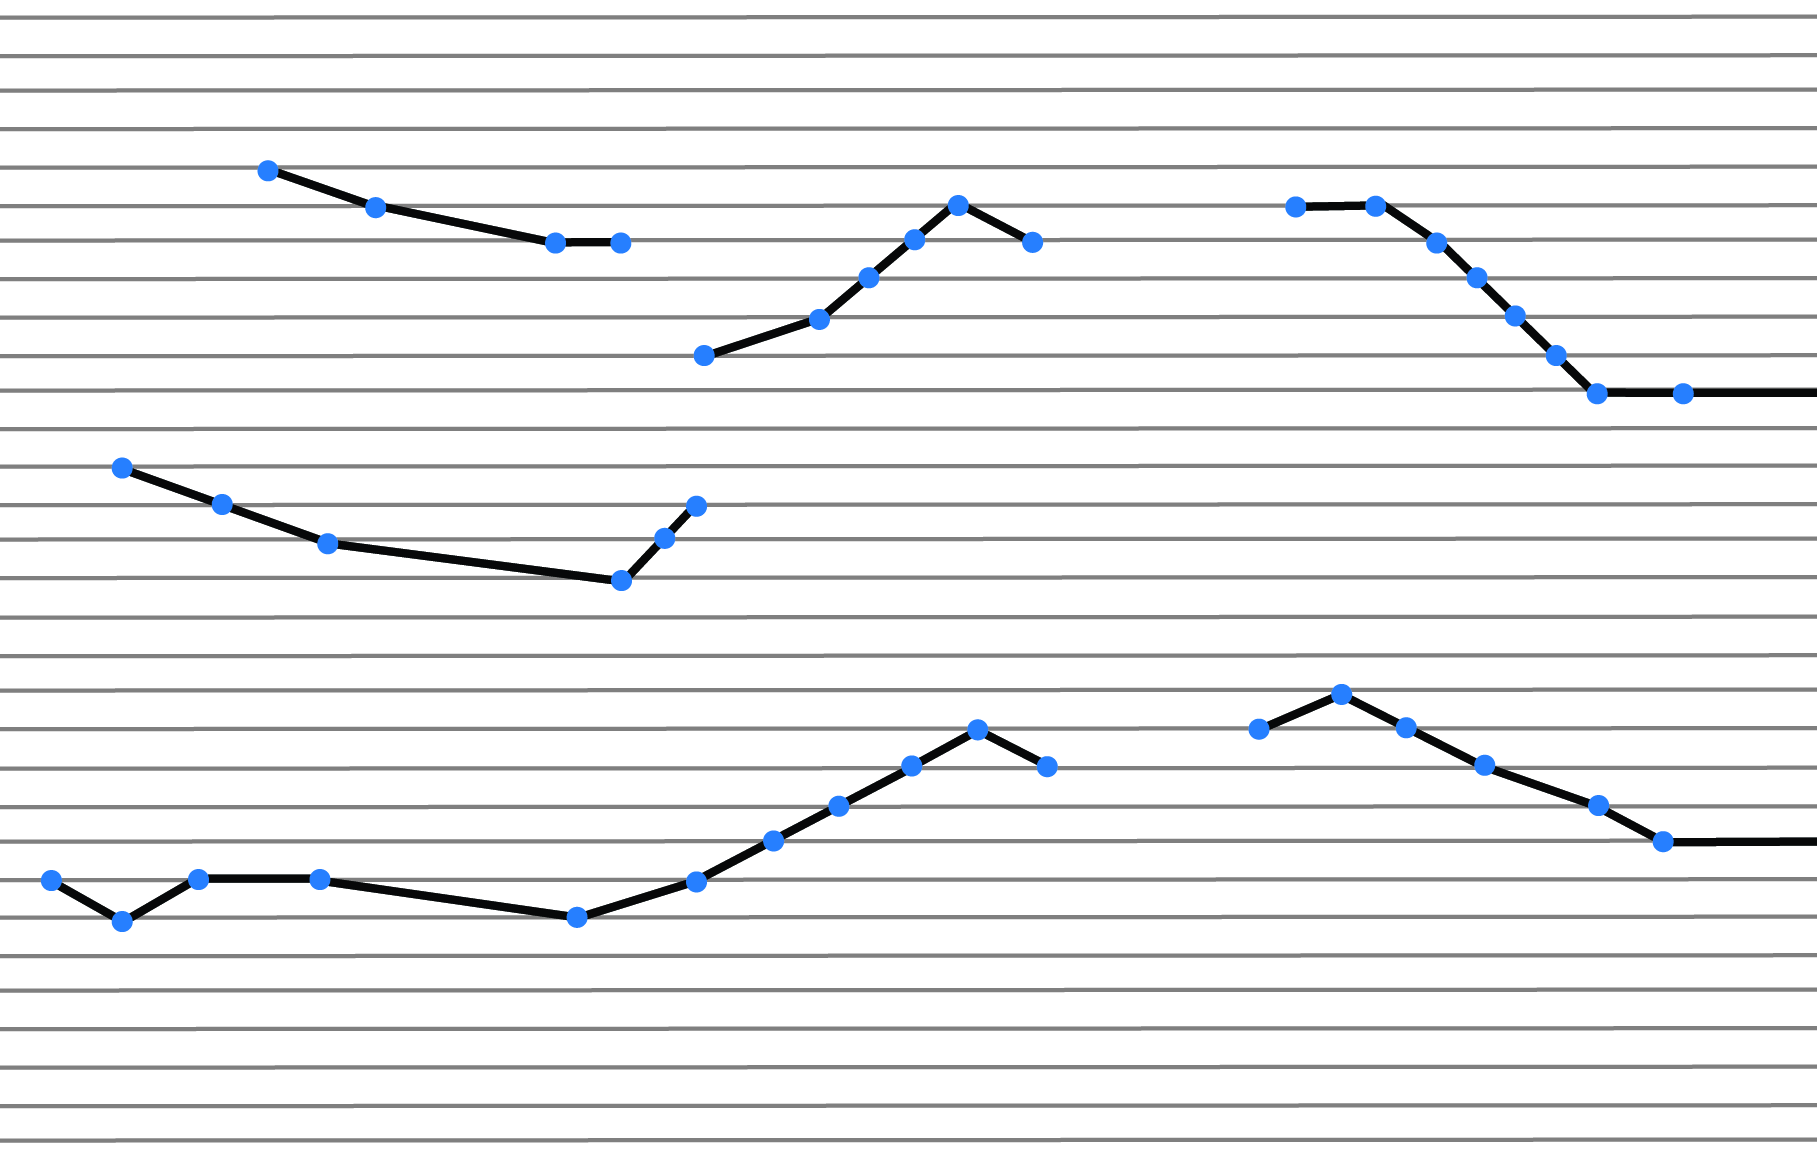
\includegraphics[width=10cm]{Chapter4/Spear3.tif} %change centimeters for resizeing
   \caption{Point selection through note modulation threshold.}
   \label{fig:example}
\end{figure}\
After these first two stages, the original data from Spear is reduced considerably by disregarding details that are not vital for the given purpose. 

The third stage, takes a note modulation threshold and averages the frequency of the pivot points to the closest given equal-tempered interval. 
The forth stage is divided in two different steps: The first step translates the lines with pivot points into a format that is compatible with the MIDI \emph{note on} and \emph{note off} paradigm. The pivot points are then considered as representing \emph{note on} messages and the \emph{note off} messages are calculated depending on whether there is a silence after the note or a new pivot point. Hence, a \emph{note off} is inserted before a new \emph{note on} or in case of a silence proceeding the pivot point. Figure 1.4 shows the glissando representation, where the notes are seen as green lines. 
\begin{figure}[htbp] %  figure placement: here, top, bottom, or page
   \centering
   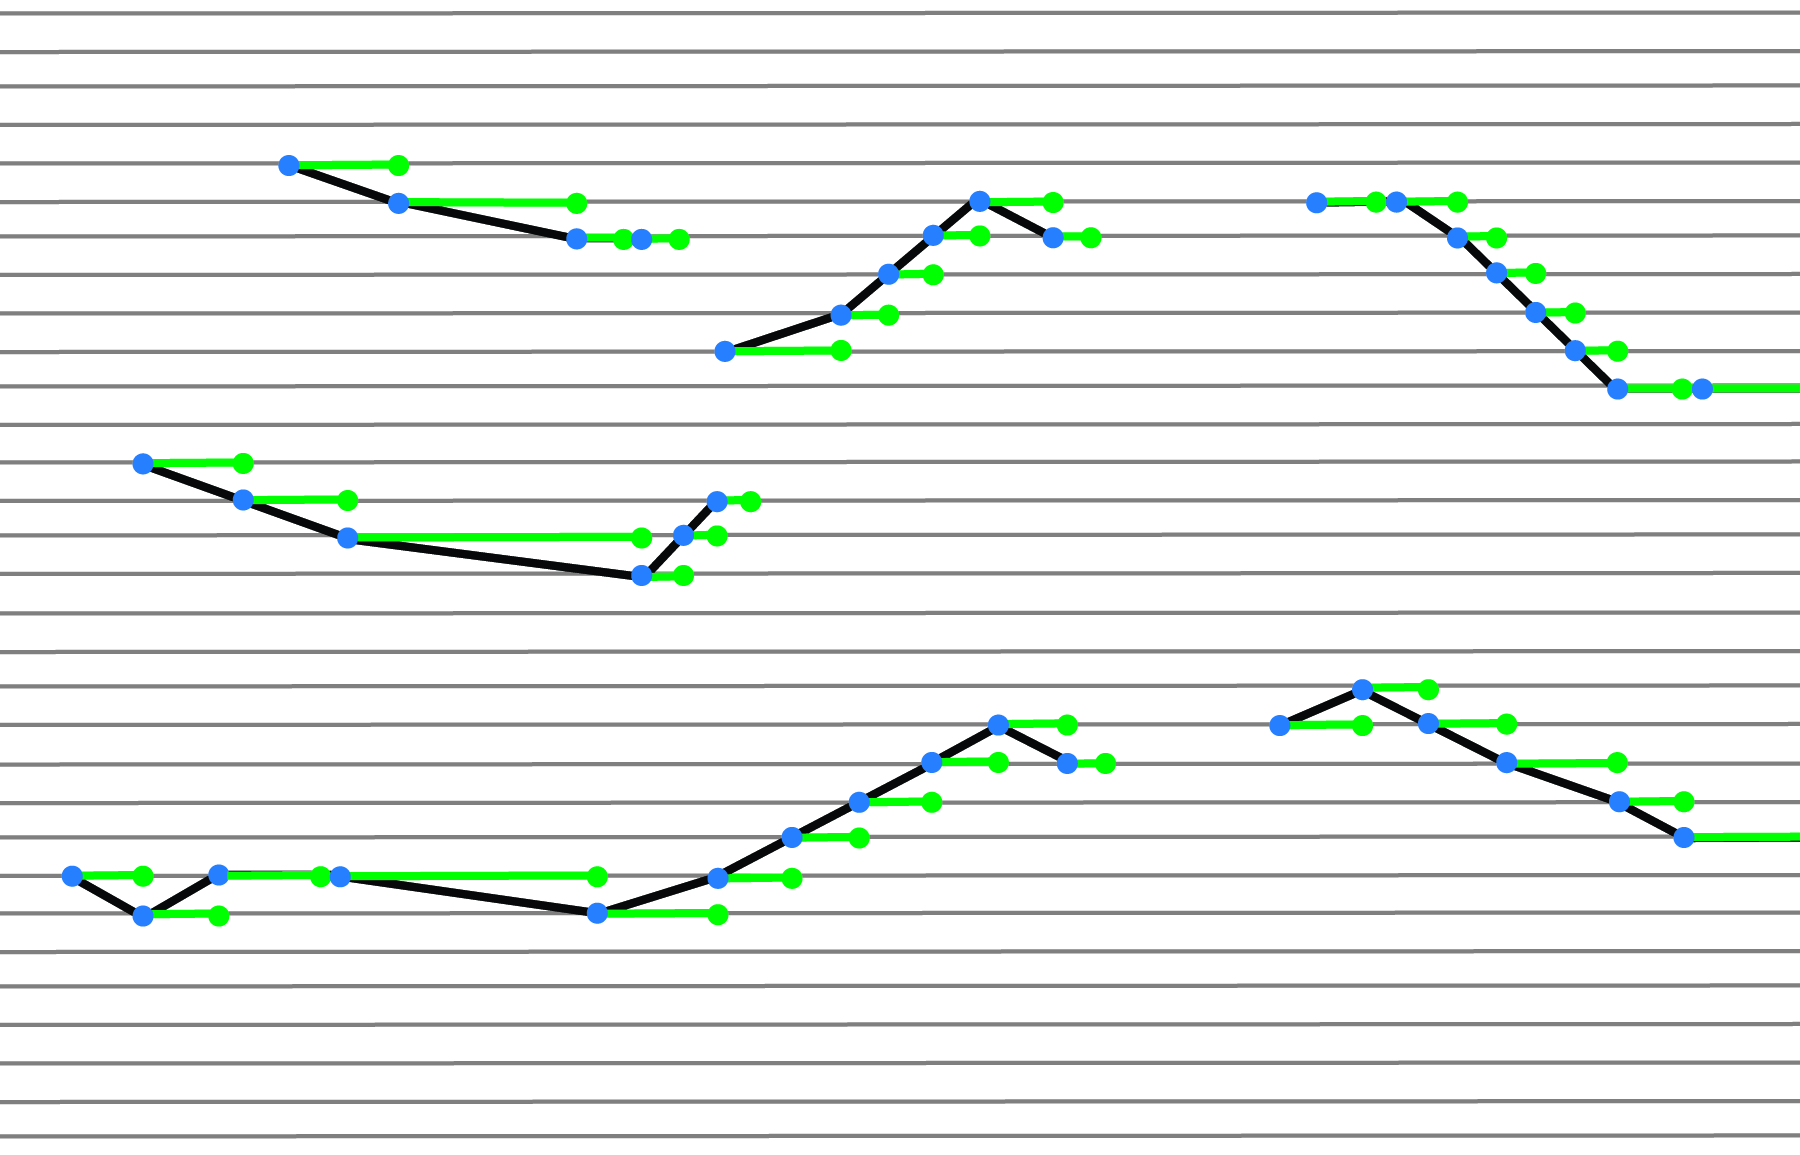
\includegraphics[width=10cm]{Chapter4/Spear4.tif} %change centimeters for resizeing
   \caption{Note representation.}
   \label{fig:example}
\end{figure}\
The results of this step can be acceded if the user's intention is to notate the partials as glissando's or if this information needs to be used to control a gradual frequency change in a synthesis definition. Lastly, the second step breaks the lines that exceed the interval set in the note modulation threshold. Therefore, it introduces new notes when the line passes the interval limit by introducing the \emph{note on} and \emph{note off} messages (as seen in Figure 1.5).


\section{Real-Time Scoring}
\subsection{AlgorithmicScore}

\section{Pre-compositional Tools}
\subsection{MIDI Mapping}
\subsection{MIDI Triggering}

\label{ch:compamp}